%% Veškerá struktura, okraje, titulní strana a balíčky jsou v upsgthesis.cls.
%% Jazyk se volí zde přes volbu třídy (english/czech); pro oboustranný tisk
%% přidejte i 'twoside,openright'.
\documentclass[czech,12pt,a4paper,twoside,openright]{upsgthesis}

%%% Údaje o práci
% Název práce v češtině (přesně podle zadání)
\ThesisTitleCZ{Název práce}
% Název práce v angličtině (přesně podle zadání)
\ThesisTitle{Thesis title}

% Typ práce
\ThesisType{bachelor}
%\ThesisType{master}
%\ThesisType{rigorous}
%\ThesisType{dissertation}
%\ThesisType{lifelong}

% Jméno autora
\ThesisAuthor{Titul. Jméno Příjmení}

% Rok odevzdání
\YearSubmitted{2026}

% Vedoucí práce: Jméno a příjmení s~tituly
\Supervisor{Titul. Jméno Příjmení}

% Studijní program a obor
\StudyProgramme{Geologie}

% Nepovinné poděkování (vedoucímu práce, konzultantovi, tomu, kdo
% zapůjčil software, literaturu apod.)
\Acknowledgements{%
Na tomto místě bych rád poděkoval vedoucímu mé bakalářské práce, panu/paní [Titul. Jméno Příjmení, Titul], za odborné vedení, cenné rady, trpělivost a čas, který mi v průběhu zpracování této práce věnoval.
}

% Abstrakt (doporučený rozsah cca 150-250 slov; nejedná se o zadání práce)
\AbstractCZ{%
Tato bakalářská práce se zabývá [hlavní téma práce, např. optimalizací logistických procesů ve vybrané firmě]. Cílem práce je [přesný cíl, např. analyzovat současný stav skladového hospodářství a navrhnout opatření ke snížení nákladů]. Teoretická část shrnuje klíčové pojmy a dosavadní poznatky v oblasti [oblast výzkumu, např. štíhlé logistiky a řízení zásob]. V praktické části je provedena [metoda, např. finanční a procesní analýza společnosti XYZ za využití metody ABC]. Na základě zjištěných nedostatků, kterými jsou zejména [hlavní problém, např. vysoká míra chybovosti a neefektivní rozmístění zboží], jsou v závěru práce formulovány konkrétní návrhy na zlepšení. Navržená řešení přinášejí [přínos, např. zkrácení doby expedice o 15\% a finanční úsporu].
}
\Abstract{%
This bachelor's thesis deals with [main topic, e.g. the optimization of logistics processes in a selected company]. The aim of the thesis is to [clear aim, e.g. analyze the current state of warehouse management and propose measures to reduce costs]. The theoretical part summarizes key concepts and current knowledge in the field of [research field, e.g. lean logistics and inventory management]. In the practical part, [method, e.g. a financial and process analysis of the company XYZ is conducted using the ABC method]. Based on the identified shortcomings, which are mainly [main problems, e.g. a high error rate and inefficient goods placement], specific proposals for improvement are formulated in the conclusion of the thesis. The proposed solutions bring [contribution, e.g. a 15\% reduction in dispatch time and financial savings].
}

% 3 až 5 klíčových slov (doporučeno)
\KeywordsCZ{klíčové slovo, další pojem, jiný důležitý termín, a ještě jeden}
\Keywords{keyword, important term, another topic, and another one}

% Výchozí soubor je bibliography.bib; podle potřeby lze zadat jiný .bib soubor.
%\Bibliography{bibliography.bib}

\begin{document}
%% Titulní strana a různé povinné informační strany
\thesisfrontmatter

\pagestyle{fancy}
%%% Jednotlivé kapitoly práce jsou pro přehlednost uloženy v samostatných souborech
\chapter*{Úvod}
\addcontentsline{toc}{chapter}{Úvod}

Úvod je povinnou částí bakalářské/diplomové práce. Úvod je uvedením do tématu. Zvolené téma rozvádí, stručně ho zasazuje do souvislostí (může zde být i popis motivace k sepsání práce) a odpovídá na otázku, proč bylo téma zvoleno. Zasazuje téma do souvislostí a zdůvodňuje jeho nutnost a aktuálnost řešení. Obsahuje explicitně uvedený cíl práce. Text cíle práce je shodný s textem, který je uveden v zadání bakalářské práce, tj. s textem, který je uveden v systému SIS a který je také uveden v části Abstrakt.

Součástí úvodu je také stručné představení postupu zpracování práce (detailně je metodě zpracování věnována samostatná část vlastního textu práce). Úvod může zahrnovat i popis motivace k sepsání práce.

Úvod k diplomové práci musí být propracovanější -- podrobněji to je uvedeno v Náležitostech diplomové práce.

Následuje několik ukázkových kapitol, které doporučují, jak by se měla závěrečná práce sázet. Primárně popisují použití \TeX{}ové šablony, ale obecné rady poslouží dobře i~uživatelům jiných systémů.

%%% Fiktivní kapitola s ukázkami sazby

\chapter{Nápověda k~sazbě}

\section{Úprava práce}

Vlastní text práce je uspořádaný hierarchicky do kapitol a podkapitol, každá kapitola začíná na nové straně. Text je zarovnán do bloku. Nový odstavec se obvykle odděluje malou vertikální mezerou a odsazením prvního řádku. Grafická úprava má být v~celém textu jednotná.

Zkratky použité v textu musí být vysvětleny vždy u prvního výskytu zkratky (v~závorce nebo v poznámce pod čarou, jde-li o složitější vysvětlení pojmu či zkratky). Pokud je zkratek více, připojuje se seznam použitých zkratek, včetně jejich vysvětlení a/nebo odkazů na definici.

Delší převzatý text jiného autora je nutné vymezit uvozovkami nebo jinak vyznačit a řádně citovat.

\section{Jednoduché příklady}

Mezi číslo a jednotku patří úzká mezera: šířka stránky A4 činí $210\,\rm mm$, což si pamatuje pouze $5\,\%$ autorů. Pokud ale údaj slouží jako přívlastek, mezeru vynecháváme: $25\rm mm$ okraj, $95\%$ interval spolehlivosti.

Rozlišujeme různé druhy pomlček:
červeno-černý (krátká),
strana 16--22 (střední),
$45-44$ (matematické minus),
a~toto je --- jak se asi dalo čekat --- vložená věta ohraničená dlouhými pomlčkami.

V~českém textu se používají \uv{české} uvozovky, nikoliv ``anglické''.

% V tomto odstavci se vlnka zviditelňuje
{
\def~{{\tt\char126}}
Na některých místech je potřeba zabránit lámání řádku (v~\TeX{}u značíme vlnovkou):
u~před\-lo\-žek (neslabičnych, nebo obecně jednopísmenných), vrchol~$v$, před $k$~kroky,
a~proto, \dots{} obecně kdekoliv, kde by při rozlomení čtenář \uv{ško\-brt\-nul}.
}

%%% Fiktivní kapitola s ukázkami tabulek, obrázků a kódu

\chapter{Tabulky, obrázky, programy}

Používání tabulek a grafů/obrázků v~odborném textu má některá společná pravidla a~některá specifická. Tabulky a grafy/obrázky neuvádíme přímo do textu, ale umístíme je buď na samostatné stránky nebo na vyhrazené místo v~horní nebo dolní části běžných stránek. \LaTeX\ se o~umístění plovoucích grafů a tabulek postará automaticky.

Grafy/obrázky a tabulky se číslují a jsou vybaveny legendou. Legenda má popisovat obsah grafu či tabulky tak podrobně, aby jim čtenář rozuměl bez důkladného studování textu práce.

Na tabulku a graf/obrázek musí být v~textu číselný odkaz (lze důrazně doporučit dynamický mechanismus křížových referencí, jený je součástí \LaTeX u). Na příslušném místě textu pak shrneme ty nejdůležitější závěry, které lze z~tabulky či grafu učinit. Text by měl být čitelný a srozumitelný i~bez prohlížení tabulek a grafů a tabulky a grafy by měly být srozumitelné i~bez podrobné četby textu.

Na tabulky a grafy odkazujeme pokud možno nepřímo v~průběhu běžného
toku textu; místo \emph{\uv{Tabulka~\ref{tab03:Nejaka} ukazuje, že
    muži jsou v~průměru o~$9,9\,\rm kg$ těžší než ženy}} raději napíšeme
\emph{\uv{Muži jsou o~$9,9\,\rm kg$ těžší než ženy (viz
    tab.~\ref{tab03:Nejaka})}}.

\section{Tabulky}

\begin{table}[htbp!]

\centering
%%% Tabulka používá následující balíčky:
%%%   - booktabs (\toprule, \midrule, \bottomrule)
%%%   - dcolumn (typ sloupce D: vycentrovaná čísla zarovnaná na
%%%     desetinnou čárku
%%%     Všimněte si, že ve zdrojovém kódu jsou desetinné tečky, ale
%%%     tisknou se čárky.

\caption{Maximálně věrohodné odhady v~modelu M.}\label{tab03:Nejaka}
\begin{tabular}{lD{.}{,}{3.2}D{.}{,}{1.2}D{.}{,}{2.3}}
\toprule
               &                & \multicolumn{1}{c}{\textbf{Směrod.}}   &  \\
\textbf{Efekt} & \multicolumn{1}{c}{\textbf{Odhad}} & \multicolumn{1}{c}{\textbf{chyba}$^a$} & \multicolumn{1}{c}{\textbf{P-hodnota}} \\
\midrule
Abs. člen     & -10.01 & 1.01 & \multicolumn{1}{c}{---} \\
Pohlaví (muž) & 9.89   & 5.98 & 0.098 \\
Výška (cm)    & 0.78   & 0.12 & <0.001 \\
\bottomrule
\multicolumn{4}{l}{\footnotesize \textit{Pozn:}$^a$ Směrodatná chyba odhadu metodou Monte Carlo.}
\end{tabular}
\end{table}

U~\textbf{tabulek} se doporučuje dodržovat následující pravidla:

\begin{itemize} %% nebo compactitem z balíku paralist
\item Vyhýbat se svislým linkám. Silnějšími vodorovnými linkami
  oddělit tabulku od okolního textu včetně legendy, slabšími
  vodorovnými linkami oddělovat záhlaví sloupců od těla tabulky a
  jednotlivé části tabulky mezi sebou. V~\LaTeX u tuto podobu tabulek
  implementuje balík \texttt{booktabs}. Chceme-li výrazněji oddělit
  některé sloupce od jiných, vložíme mezi ně větší mezeru.
\item Neměnit typ, formát a význam obsahu políček v~tomtéž sloupci
  (není dobré do téhož sloupce zapisovat tu průměr, onde procenta).
\item Neopakovat tentýž obsah políček mnohokrát za sebou. Máme-li
  sloupec \textit{Rozptyl}, který v~prvních deseti řádcích obsahuje
  hodnotu $0,5$ a v~druhých deseti řádcích hodnotu $1,5$, pak tento
  sloupec raději zrušíme a vyřešíme to jinak. Například můžeme tabulku
  rozdělit na dvě nebo do ní vložit popisné řádky, které informují
o~nějaké proměnné hodnotě opakující se v~následujícím oddíle tabulky
  (např. \emph{\uv{Rozptyl${}=0,5$}} a níže \emph{\uv{Rozptyl${}=
      1,5$}}).
\item Čísla v~tabulce zarovnávat na desetinnou čárku.
\item V~tabulce je někdy potřebné používat zkratky, které se jinde
nevyskytují. Tyto zkratky můžeme vysvětlit v~legendě nebo
v~poznámkách pod tabulkou. Poznámky pod tabulkou můžeme využít i
k~podrobnějšímu vysvětlení významu  některých sloupců nebo hodnot.
\end{itemize}


\section{Obrázky}

\begin{figure}[htbp!]\centering
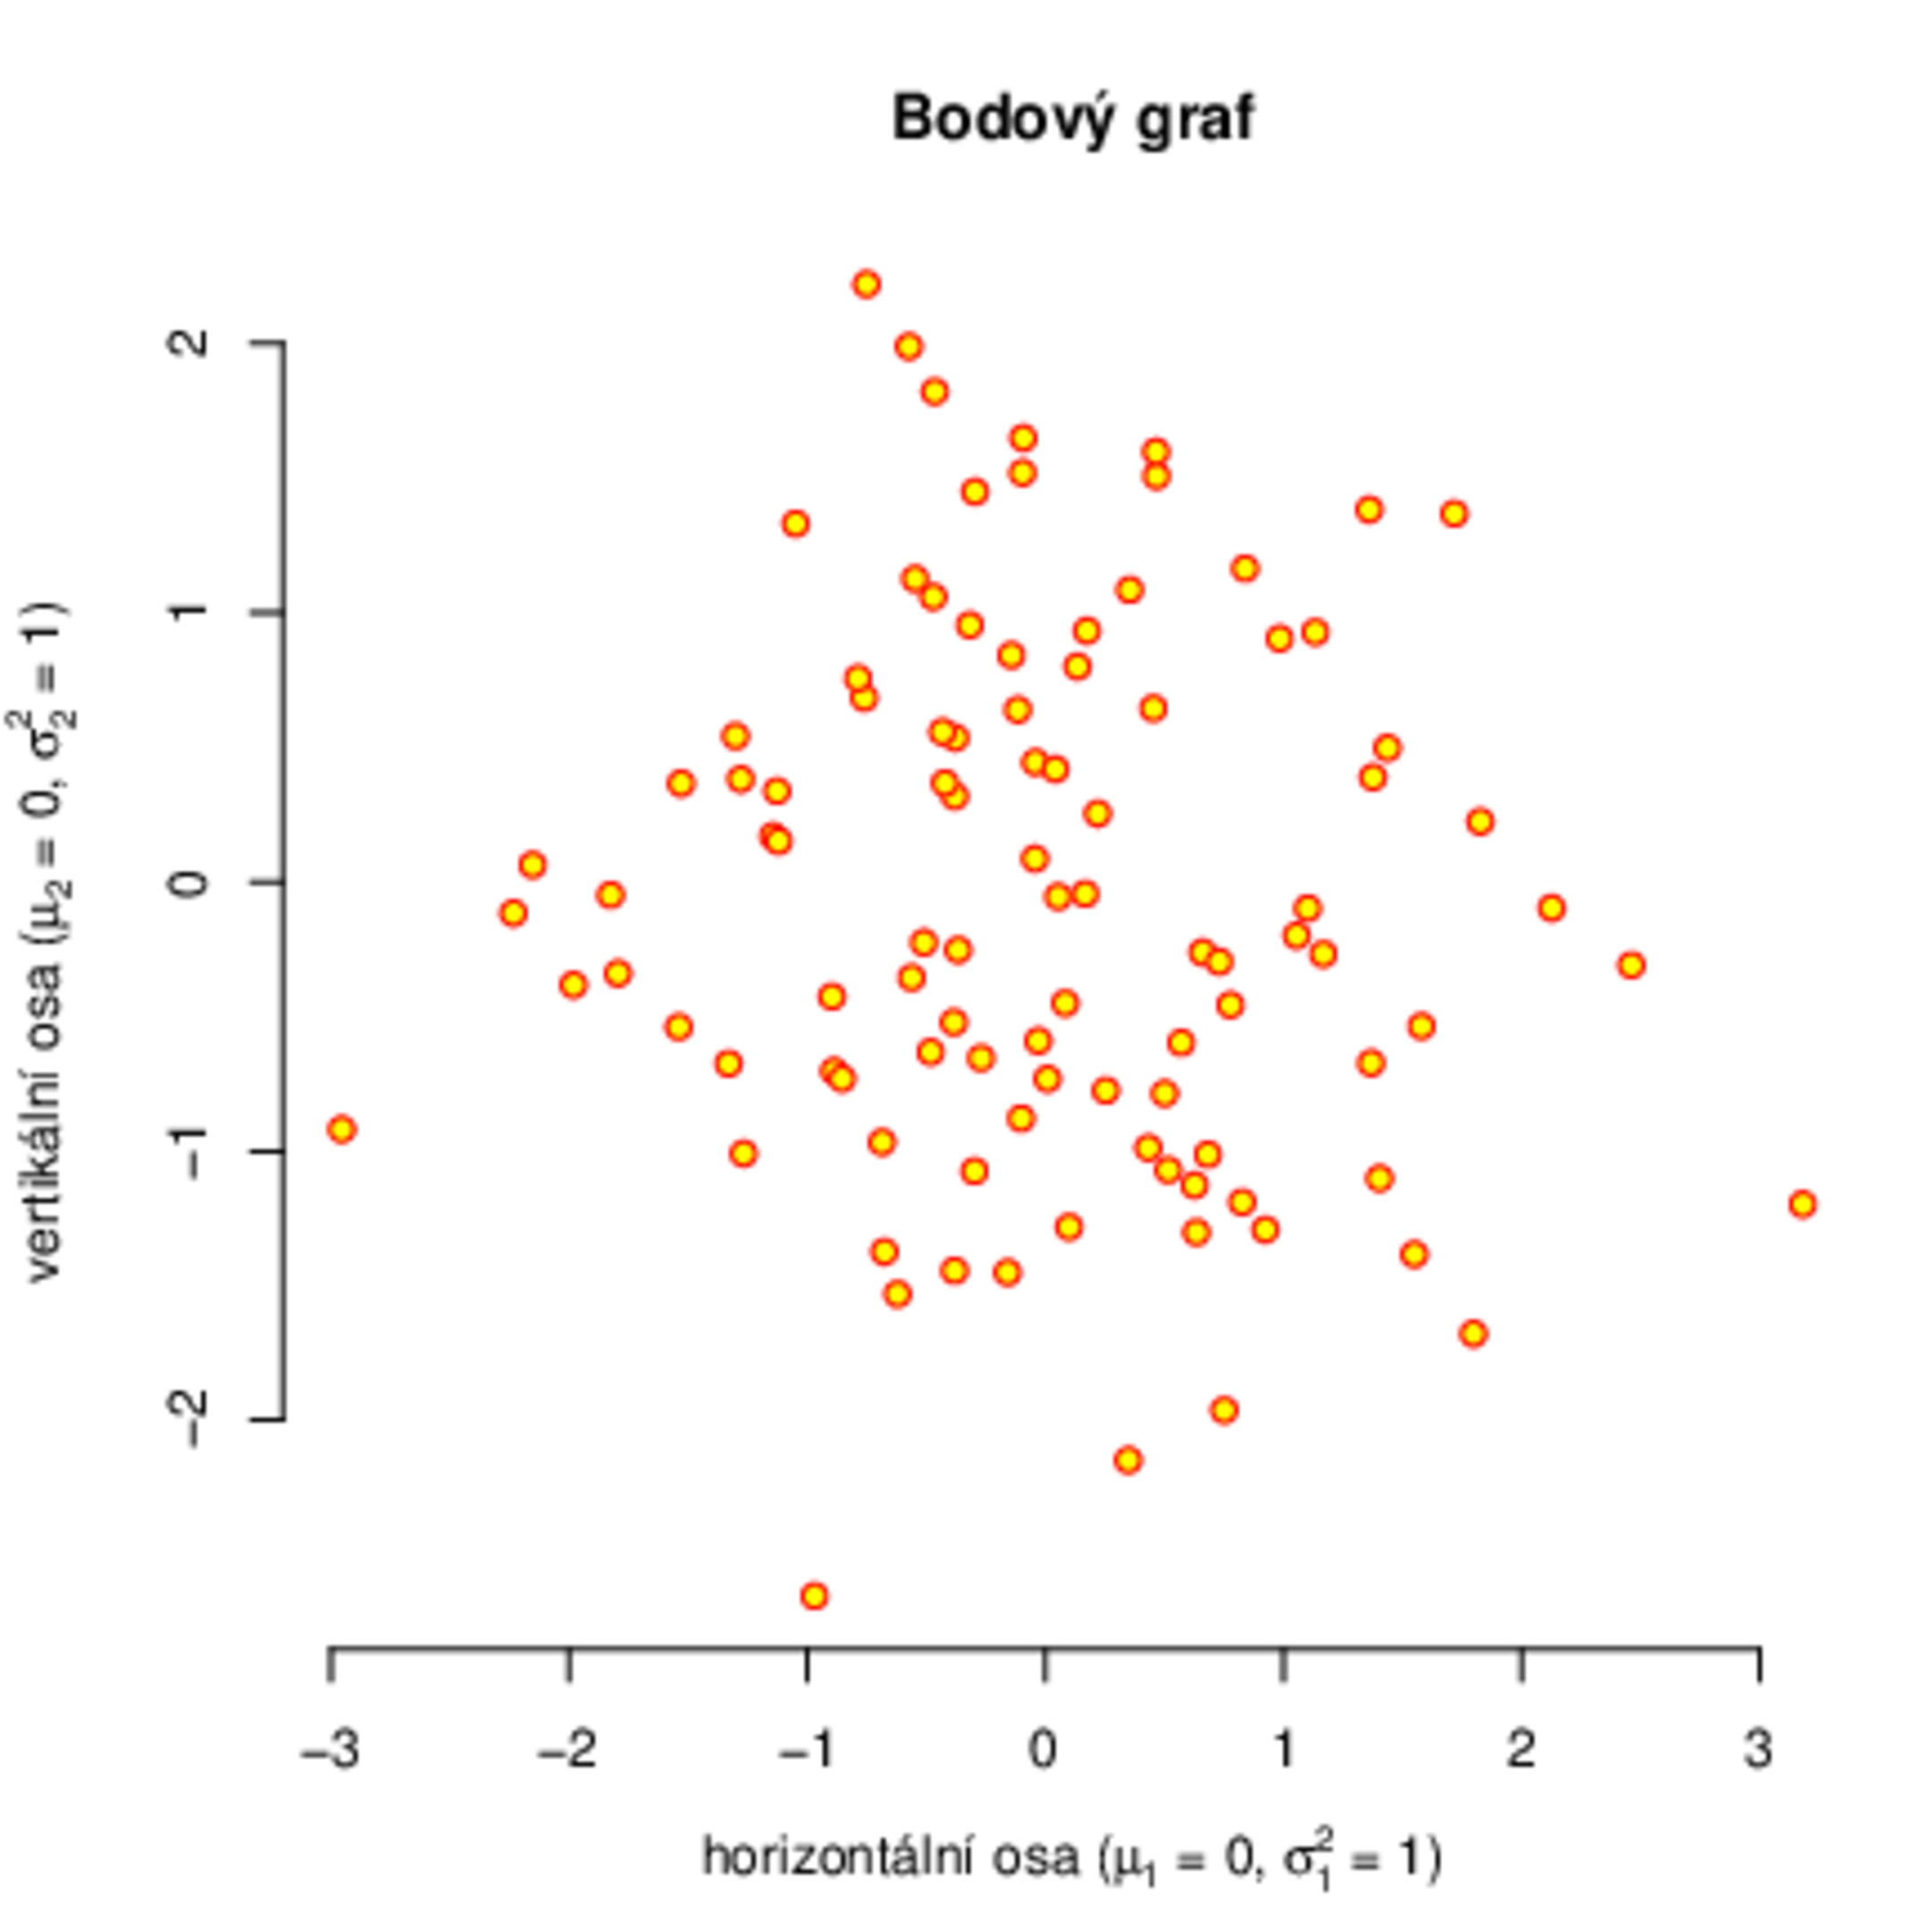
\includegraphics[width=.66\textwidth]{figures/example-fig01}
% Příponu není potřeba explicitně uvádět, pdflatex automaticky hledá pdf.
% Rozměry také není nutné uvádět.
\caption{Náhodný výběr z~rozdělení $\mathcal{N}_2(\boldsymbol{0},\,I)$.}
\label{obr03:Nvyber}
\end{figure}

Několik rad týkajících se obrázků a grafů.

\begin{itemize}
\item Graf by měl být vytvořen ve velikosti, v~níž bude použit
  v~práci. Zmenšení příliš velkého grafu vede ke špatné čitelnosti
  popisků.
\item Osy grafu musí být řádně popsány ve stejném jazyce, v~jakém je
  psána práce (absenci diakritiky lze tolerovat). Kreslíme-li graf
  hmotnosti proti výšce, nenecháme na nich popisky \texttt{ht} a
  \texttt{wt}, ale osy popíšeme \emph{Výška [cm]} a~\emph{Hmotnost
    [kg]}. Kreslíme-li graf funkce $h(x)$, popíšeme osy $x$ a $h(x)$.
  Každá osa musí mít jasně určenou škálu.
\item Chceme-li na dvourozměrném grafu vyznačit velké množství bodů,
  dáme pozor, aby se neslily do jednolité černé tmy. Je-li bodů mnoho,
  zmenšíme velikost symbolu, kterým je vykreslujeme, anebo vybereme
  jen malou část bodů, kterou do grafu zaneseme. Grafy, které obsahují
  tisíce bodů, dělají problémy hlavně v~elektronických dokumentech,
  protože výrazně zvětšují velikost souborů.
\item Budeme-li práci tisknout černobíle, vyhneme se používání barev.
  Čáry roz\-li\-šu\-je\-me typem (plná, tečkovaná, čerchovaná,\ldots), plochy
  dostatečně roz\-díl\-ný\-mi intensitami šedé nebo šrafováním. Význam
  jednotlivých typů čar a~ploch vysvětlíme buď v~textové legendě ke
  grafu anebo v~grafické legendě, která je přímo součástí obrázku.
\item Vyhýbejte se bitmapovým obrázkům o~nízkém rozlišení a zejména
  JPEGům (zuby a kompresní artefakty nevypadají na papíře pěkně).
  Lepší je vytvářet obrázky vektorově a vložit do textu jako PDF (Pozor na problém s PDF/A, viz. kapitola~\ref{kap:pdfa}).
\end{itemize}


\section{Zdrojové kódy}
Algoritmy, výpisy programů a popis interakce s~programy je vhodné odlišit od ostatního textu. Třída \texttt{upsgthesis.cls} pro to definuje prostředí \texttt{code} postavené na balíčku \texttt{listings}, se zvýrazněním syntaxe podle jazyka zadaného jako jeho nepovinný parametr, např.\ \verb|\begin{code}[Python]|. Bez parametru se text sází obyčejně, bez zvýrazňování -- hodí se to např. pro přepis výstupu z konzole, jako v následující ukázce. Delší nebo doplňkové zdrojové kódy patří spíše do přílohy (viz příloha~\ref{app:kody}, kde je i ukázka zvýrazněného kódu v Pythonu).

\begin{code}
> mean(x)
[1] 158.90
> objekt$prumer
[1] 158.90
\end{code}

Balíček \texttt{listings} je mnohem bohatěji konfigurovatelný, než co tato šablona standardně nastavuje -- viz jeho dokumentace, nebo:
\begin{itemize}
\item \url{https://en.wikibooks.org/wiki/LaTeX/Source_Code_Listings}
\item \url{https://www.overleaf.com/learn/latex/Code_listing#Using_listings_to_highlight_code}
\end{itemize}


\section{Sazba matematiky}
Proměnné sázíme kurzívou (to \TeX{} v~matematickém módu dělá sám, ale
nezapomínejte na to v~okolním textu a také si matematický mód zapněte).
Názvy funkcí sázíme vzpřímeně. Tedy například:
$\textrm{var} (X) = \textsf{E~} X^2 - \bigl(\textsf{E~} X \bigr)^2$.

Zlomky uvnitř odstavce (třeba $\frac{5}{7}$ nebo $\frac{x+y}{2}$) mohou
být příliš stísněné, takže je lepší sázet jednoduché zlomky s~lomítkem:
$5/7$, $(x+y)/2$.

Možnosti \LaTeX u pro sazbu matematiky jsou sice bohaté, ale je možné, že v některých specifických situacích nebudou postačovat. Proto lze doporučit k použití balíčky American Mathematical Society (AMS). Ve třídě \texttt{upsgthesis.cls} jsou standardně zaváděny balíčky \texttt{amsmath}, \texttt{amsfonts} a \texttt{amsthm}. Pro proniknutí do jejich možností poslouží:
\begin{itemize}
\item Math Extension with AMS\LaTeX\ -- \url{http://ptgmedia.pearsoncmg.com/images/0321173856/samplechapter/kopkach15.pdf}
\item \url{https://www.overleaf.com/learn/latex/Aligning_equations_with_amsmath}
\item Math Mode -- \url{http://tex.loria.fr/general/Voss-Mathmode.pdf}
\item More Math into LaTeX -- \url{http://tug.ctan.org/info/Math_into_LaTeX-4/Short_Course.pdf}
\end{itemize}

%%% Fiktivní kapitola s ukázkami citací

\chapter{Práce s literaturu}

Šablona předpokládá použití bibliografické databáze z důvodu větší flexibility. Použití bibliografické databáze není nutnou podmínkou, lze si vystačit i se standardním prostředím \texttt{thebibliography}. V takovém případě je však zapotřebí provést zásahy do třídy \texttt{upsgthesis.cls} a hlavního souboru, jak je uvedeno dále.

\section{Použití bibliografické databáze}

\begin{enumerate}
\item\textbf{Změna názvu databáze}\\
V šabloně se předpokládá databáze uložená v souboru \texttt{bibliography.bib}. Pokud se databáze jmenuje jinak, pak je nutné ve třídě \texttt{upsgthesis.cls} změnit hodnotu parametru příkazu \verb'\addbibresource'.
\item\textbf{Změna citačního stylu}\\
Standardně se citace v textu uvádějí v číselné variantě. Na použití kombinace příjmení a roku lze snadno přepnout změnou ve třídě \texttt{upsgthesis.cls}, kde se prohodí komentářový znak v parametrech pro balíček \texttt{biblatex}.
\end{enumerate}


\section{Použití prostředí \texttt{thebibliography}}
\begin{enumerate}
\item Ve třídě \texttt{upsgthesis.cls} vymazat na počátku tyto řádky:
\begin{verbatim}
%%% Nastavení pro použití samostatné bibliografické databáze
\RequirePackage[
   backend=biber
  ,style=iso-authoryear %iso-numeric
  ,sortlocale=cs_CZ
  ,bibencoding=UTF8
  %,block=ragged
]{biblatex}
\addbibresource{bibliography.bib}
\end{verbatim}
\item Ve třídě \texttt{upsgthesis.cls} upravit příkaz \verb'\thesisbibliography', odstranit v něm \verb'\printbibliography' a nahradit ho prostředím \texttt{thebibliography}.
\end{enumerate}


\section{Jak citovat v textu}
\begin{center}
\begin{tabular}{l@{~~$\longrightarrow$~~}l}
\verb|\cite{Cermak2018}|&\cite{Cermak2018}\\
\verb|\cite{Hladik2018,Jasek2018}|&\cite{Hladik2018,Jasek2018}\\
\verb|\cite[kap. 3]{Pecakova2018}|&\cite[kap. 3]{Pecakova2018}\\
\end{tabular}
\end{center}

%%% Fiktivní kapitola s instrukcemi k PDF/A

\chapter{Formát PDF/A}\label{kap:pdfa}

Elektronická podoba závěrečných
prací musí být odevzdávána ve formátu PDF/A úrovně 1a nebo 2u. To jsou
profily formátu PDF určující, jaké vlastnosti PDF je povoleno používat,
aby byly dokumenty vhodné k~dlouhodobé archivaci a dalšímu automatickému
zpracování. Dále se budeme zabývat úrovní 2u, kterou sázíme \TeX{}em.

Mezi nejdůležitější požadavky PDF/A-2u patří:

\begin{itemize}

\item Všechny fonty musí být zabudovány uvnitř dokumentu. Nejsou přípustné
odkazy na externí fonty (ani na \uv{systémové}, jako je Helvetica nebo Times).

\item Fonty musí obsahovat tabulku ToUnicode, která definuje převod z~kódování
znaků použitého uvnitř fontu to Unicode. Díky tomu je možné z~dokumentu
spolehlivě extrahovat text.

\item Dokument musí obsahovat metadata ve formátu XMP a je-li barevný,
pak také formální specifikaci barevného prostoru.

\end{itemize}

Tato šablona používá balíček {\tt pdfx,} který umí \LaTeX{} nastavit tak,
aby požadavky PDF/A splňoval. Metadata v~XMP generuje {\tt pdfx} automaticky
(na vygenerovaný soubor se můžete podívat v~{\tt pdfa.xmpi}); požadavek
PDF/A na přítomnost XMP metadat je tím splněn bez nutnosti spravovat
další soubor.

Správnost PDF/A lze zkontrolovat pomocí on-line validátoru: \url{https://www.pdf-online.com/osa/validate.aspx/}.

Pokud soubor nebude validní, mezi obvyklé příčiny patří používání méně
obvyklých fontů (které se vkládají pouze v~bitmapové podobě a/nebo bez
unicodových tabulek) a vkládání obrázků v~PDF, které samy o~sobě standard
PDF/A nesplňují.

Je pravděpodobné, že se to týká obrázků vytvářených mnoha různými programy.
V~takovém případě se můžete pokusit obrázek do zkonvertovat do PDF/A pomocí
GhostScriptu, například takto:

\begin{verbatim}
        gs -q -dNOPAUSE -dBATCH
           -sDEVICE=pdfwrite -dPDFSETTINGS=/prepress
           -sOutputFile=vystup.pdf vstup.pdf
\end{verbatim}

% \include{...}
% \include{...}
\chapter*{Závěr}
\addcontentsline{toc}{chapter}{Závěr}

Závěr je povinnou částí bakalářské/diplomové práce. Obsahuje shrnutí práce a vyjadřuje se k míře splnění cíle, který byl v práci stanoven, případně shrnuje odpovědi na otázky, které byly položeny v úvodu práce. 

Závěr k diplomové práci musí být propracovanější -- podrobněji to je uvedeno v Náležitostech diplomové práce v rámci Intranetu pro studenty FIS.

Závěr je vnímán jako kapitola (chapter), která začíná na samostatné stránce a která má název Závěr.  Název Závěr se nečísluje. Samotný text závěru je členěn do odstavců.

%%% Seznam použité literatury
\thesisbibliography

%%% Přílohy k bakalářské práci, existují-li. Každá příloha musí být alespoň jednou
%%% odkazována z vlastního textu práce. Přílohy se číslují.
\thesisappendices
\chapter{Zdrojové kódy}\label{app:kody}

Následující skript v jazyce Python spouštěný z příkazové řádky načte body ze souboru GPX a přidá je jako lokality do databáze SDB; ukazuje typický krátký nástroj pro zpracování dat.

\begin{code}[Python]
from typing import Annotated
import typer
from gpx import read_gpx
from apsg.database import SDBSession


def format_name(name):
    prefix = "".join(c for c in name if not c.isdigit())
    suffix = "".join(c for c in name if c.isdigit())
    return f"{prefix}{int(suffix):03d}"


def main(
    sdb: Annotated[str, typer.Argument(help="path of SDB database.")],
    file: Annotated[str, typer.Argument(help="path of GPX file.")],
    fixname: bool = False,
):
    """
    Add sites from gpx file to SDB

    Examples:
        $ add_from_gpx.py dest.sdb file.gpx
        $ add_from_gpx.py dest.sdb file.gpx --fixname

    """
    db = SDBSession(sdb)
    gpx = read_gpx(file)
    unit = db.unit("Default")
    for wpt in gpx.wpt:
        site = db.site(
            wpt.name,
            unit=unit, x_coord=float(wpt.lon), y_coord=float(wpt.lat)
        )
        print(f"{site} added")

    confirm = input("OK? [y/N] ")
    if confirm in ["Y", "y"]:
        db.commit()
        db.close()
        print("Done.")
    else:
        print("Canceled.")


if __name__ == "__main__":
    typer.run(main)
\end{code}


% \include{...}
% \include{...}

\end{document}
